\chapter{Results}
- Each test is run with several basic values that remain unchanged unless otherwise specified: 
- We use 5-hit events, with all 5 hits used in the reconstruction, energy and spatial noise at close to real values (.22 energy noise, 1 mm of spatial noise) and the predicted noise at the same levels
- Each error bar is calculated under the assumption of Gaussian noise, with a p-value of .005
- 

\section{Power}

- We use the WITRN U2 USB Power Monitor to test the power when it's idle and when it's running
- Once plugged in, it displays the average power used and the max power used
- We tested it for a half hour in idle mode - x watts
- We tested it after running our program for 5 minutes - x watts
- We tested it after running for about a half hour - x watts
- This isn't the final hardware, so it probably wouldn't mean much to report the exact values, but the hardware on the APT will be similar, so we expect it to be a good estimate
- draws about 2-4 watts when it's running
- this is well below the 50W we needed to keep under (from Jim), so I think we're good

\section{Precision}
- on a pi, single precision is 32-bit and double precision is 64-bit
- single precision: $3.848x105 \pm 0.513x10^5$ photons/sec vs. double: $5.076x10^5 \pm 0.698x10^5$ photons/sec
- x trials, x photons per trial
- accuracy: 86.12\% vs 86.15\% for accuracy. Not enough that it would make a huge difference for our purposes since our measurements' noise threshold will probably account for a greater error than that.
- since the pi is an in-order processor, it runs comparatively slower with double-precision values than if it were an out-of-order processor
- Using double-precision values reduces rounding error, but it does not give us enough of an increase in accuracy to warrant the reduction in speed.

\section{Parallelism}
- Tested on Cassini because it has more cores
- We run our algorithm on different numbers of cores and calculate the speedup of each trial
- We are using a constant workload for each run, so the speedup in the latency is the sequential execution time divided by the parallel execution time.
- The speedup in throughput is the number of cores used for each run multiplied by the speedup in latency for each run.
- Shows an overall linear trend in speedup, which means that our program has good scalability.

\begin{figure}
    \centering
    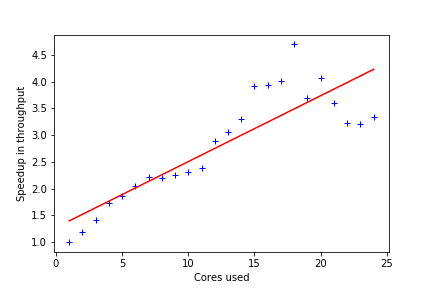
\includegraphics[width=0.7\textwidth]{graphs/Cassini_throughput_speedup.png}
    \caption{Speedup of reconstruction algorithm in throughput.}
    \label{fig:through_speedup}
\end{figure}

\section{Differing numbers of hits}
- Accuracy peaks at about 5 hits, which is interesting
- Speed looks like it goes down exponentially with number of hits, which was also expected (but better than factorial time?)

\section{Hits used in reconstruction}
- Accuracy seems to tail off around 6-8 hits for the toy model
- photons/sec goes down pretty linearly as we increase hits used
- if we get better simulations with Geant we can change the number of hits we use based on the number of hits we receive to maximize our accuracy while minimizing the time spent on each photon

\begin{figure}
    \centering
    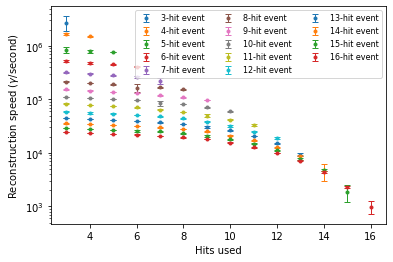
\includegraphics[width=0.7\textwidth]{graphs/pi_hits_v_hitsUsed_speed_final.png}
    \caption{Decrease in throughput with hits used in reconstruction}
    \label{fig:hits_v_hitsUsed}
\end{figure}

\section{p-value}
- visible correlation, but try to get a better one
- speed idk, could increase could decrease, get better error values

\section{$\eta$-tolerance}
- found no real correlation, just noise

\section{Estimated Noise}
- estimated energy noise has a clear downward trend, but over a pretty small range of accuracies
- spatial noise not so much, perhaps increase the range

\section{Simulated Noise}
- helps with proof of concept
- we expect accuracy to go down with increased noise, and it does for both